\documentclass[11pt,letterpaper]{article}
\usepackage[margin=0.63in,top=0.77in,bottom=0.66in,headheight=15pt,headsep=16pt]{geometry}
\usepackage[T1]{fontenc}
\usepackage{helvet}
\renewcommand{\familydefault}{\sfdefault}
\usepackage{amsmath,amssymb,array,booktabs,enumitem,tikz,fancyhdr}
\usetikzlibrary{arrows.meta}
\usepackage[hidelinks]{hyperref}
\pagestyle{fancy}\fancyhf{}
\fancyhead[L]{\small Week 60 / Take it or pass / Adult guide}
\fancyfoot[L]{\footnotesize Bellingham Math Circle / Week 60 / W60-FAC-v1}
\fancyfoot[R]{\footnotesize\thepage}
\renewcommand{\headrulewidth}{0.4pt}\renewcommand{\footrulewidth}{0pt}
\setlength{\parindent}{0pt}\setlength{\parskip}{6pt}
\setlist[itemize]{leftmargin=16pt,itemsep=2pt,topsep=3pt}
\setlist[enumerate]{leftmargin=18pt,itemsep=2pt,topsep=3pt}
\setlength{\tabcolsep}{5pt}\renewcommand{\arraystretch}{1.14}
\pdfinfoomitdate=1\pdftrailerid{}
\newcommand{\topic}[1]{\par\textbf{\large #1}\par}
\newcommand{\task}[2]{\par\textbf{Problem #1 / #2}\par}
\newcommand{\hint}[1]{\textbf{Hints, in order.} #1\par}
\newcommand{\word}[1]{\ensuremath{(#1)}}
\begin{document}

\topic{The mathematical destination}
\textbf{Finite-horizon stopping theorem.} Fix the number of offers before a round.
Every offer is an independent draw from the same known finite distribution of scores.
Take the current score and end, or pass it permanently; the final offer must be
taken, including zero. Only the accepted score counts. There are no fees or recall.
The objective is the \emph{expected accepted score}: the probability-weighted
average over possible rounds.

Let $V_m$ be the best average \emph{before seeing} any of $m$ remaining offers.
If $X$ is one fresh offer, then
\[
 V_1=\mathbb E[X],\qquad V_m=\mathbb E[\max\{X,V_{m-1}\}]\quad(m>1).
\]
With $m>1$ offers left \emph{including the current offer} $x$, take when
$x>V_{m-1}$ and pass when $x<V_{m-1}$. At equality either choice is optimal.
The last offer has no pass option. The recurrence compares taking with the best
\emph{whole remaining plan}, rather than just the next draw.

Replacement and independence make every passed history irrelevant to the
future distribution. Backward induction bounds every legal plan, even one that
remembers earlier offers or randomizes its decisions. For tickets $0,4,6$,
\[
 V_1=10/3,\qquad V_2=40/9,\qquad V_3=134/27.
\]
Thus take a current $4$ with two offers left, but pass it with three.
For $0,3,6$ with two offers, taking or passing $3$ ties; both optimal plans total
$36$ on nine cases. More offers never lower the optimum. For any nonconstant
finite bag they strictly raise it at each finite horizon; a constant-score bag
gives equality. Proofs appear on pages 6--8.

\textbf{Limits.} A known bag without replacement requires its remaining inventory
as part of the state. Recall, changing probabilities, fees, an unknown horizon,
or an objective such as selecting the overall largest offer require a different
model. This is expected-score stopping, not the rank-only secretary problem.
The mathematical iid assumption is stronger than merely returning a physical
ticket: the proposed mixing procedure needs rehearsal.

\textbf{Experiments, conjectures and explanations.} Six played rounds may suggest
a rule. All equally likely full words evaluate a fixed rule exactly. A complete
policy audit or backward argument establishes optimality. A favorable sample
does not certify a better average. An expected score is not a promised score in
the next round or short batch.

\textbf{Actual student map: one seven-page packet, W60-S-v2.}
\begin{center}\small
\begin{tabular}{@{}p{1.15in}p{1.55in}p{4.23in}@{}}\toprule
Student pages & Band and route & What children can discover \\\midrule
1--3 and 6 & Grades 3--5; concrete core & Invent/apply rules; construct opposite samples; pool nine/27 cases; compare totals; find the tie in a new bag. \\
4--5 and 7 & Grades 4--5; continuation & Compare continuation averages; prove a bound for history-dependent plans; change horizons; explain extra offers. \\
No new pages & K--1 & Use a separate familiar activity. This guide adds no K--1 stopping theme. \\\bottomrule
\end{tabular}\end{center}
Adult reading and addition can support the core. Children must compare scores,
count turns, retain take/pass and a deadline, and apply a fixed rule. Upper work
needs averages, fractional comparisons and readiness for a branching argument.
Success can be one sound investigation; the packet can support several visits.

\newpage
\topic{Prepare for eleven children and three anchored adults}
\textbf{KK11:} two kindergartners and two first graders with the parent volunteer.
\textbf{3333:} four third graders with a mathematician, in two pairs.
\textbf{445:} two fourth graders and one fifth grader with the organizer;
a pair and a rotating referee. Adults stay at their tables. This staffing is
part of the proposed plan, not a tested independence claim.

\textbf{Three older-table playing kits.} Per kit: one opaque bag; three equal
cardstock randomizing tickets $0,4,6$ (about $40\times60$ mm); a separate visible
distribution list; four counters; one erasable offer display; one TAKE and one
PASS place; pencil and eraser. Total: three bags, nine tickets, three lists,
12 counters, three displays, six action places, three pencils and three erasers.
Keep one spare three-ticket
set, four counters, one pencil and one eraser. All ticket backs, thicknesses,
edges and sizes must be indistinguishable by sight or touch while drawing.

The \emph{randomizing ticket} always goes back into the bag. The \emph{display}
keeps the offered number visible while it is returned and mixed. Taking places
the display at TAKE and ends the round; it does not remove a bag ticket.
Passing places it at PASS, then the display is cleared for the next offer.
The partner prevents reclaiming passed offers. Check whether one counter
remains \emph{while deciding}; remove a counter only \emph{after} the decision.

For later new bags, prepare three replacement sets of $0,3,6$ and three of
$0,5,6$: nine tickets per distribution, 18 additional tickets. Switch whole
labelled sets and update the visible list; do not mix distributions. Reuse sets across visits.
For the shared demonstration, have one separate three-ticket set $1,2,5$.
For the optional average example, have nine cubes and three sharing places.

\textbf{Print single-sided US Letter at 100\%. Give one page at a time.}
\begin{center}\small
\begin{tabular}{@{}p{1.6in}p{4.8in}r@{}}\toprule
Print & Allocation & Sheets \\\midrule
Student page 1 & Seven older children plus one spare & 8 \\
Pages 2, 3, 6 on paper & One working sheet per kit, plus one spare of each page & 12 \\
Pages 4, 5, 7 on paper & Three upper children plus one spare of each; keep for readiness/later & 12 \\
Pages 2, 3, 6 on cardstock & One complete table set for each older table: two copies of each & 6 \\
Pages 2, 3, 6 spare cardstock & One spare copy of each; leave uncut until needed & 3 \\
Adult guide & One per adult & 3 guides \\\bottomrule
\end{tabular}\end{center}
Each table's supplied cards are nine $0/4/6$ pairs, 27 $0/4/6$ triples,
nine $0/3/6$ pairs and nine $0/5/6$ pairs: \textbf{54 cards per table, 108 cut
cards altogether}; the uncut spare set supplies another 54. Cut dashed borders.
Label four envelopes by bag and word length. Children share and partition a
table's complete set; each child need not copy or score all 27 cards. Allow
roughly 15--25 minutes for copying, cutting and sorting; this estimate is untested.

\textbf{KK11 is a separate prior option.} Resume unused Week 1 K--1 tiling pages
1--2 (F01-K-v4), with the current Week 1 adult guide. Print four copies of each
plus one spare: ten sheets. For four child kits plus one spare, plan 30 small
blue rhombi, 60 green triangles, 15 purple trapezoids, ten red trapezoids and ten
yellow hexagons; larger pieces stay aside. Reuse pieces between shapes.
Check a printed triangle edge against a real small block. This is previously
available tiling, not new Week 60 coverage; confirm what these children already
used before choosing it. The old guide's 3/3/1 roster is historical.

\newpage
\topic{A flexible hour and the handling pretest}
\begin{center}\small
\begin{tabular}{@{}p{0.65in}p{6.17in}@{}}\toprule
Minutes & Proposed route \\\midrule
0--5 & Movement/running around. \\
5--7 & Handle tickets, counters and action places freely; handle blocks at KK11. \\
7--10 & Brief shared legal-round demonstration below. KK11 then has a 30-second familiar placement reminder at its table. \\
10--25 & Older pairs play Problem 1, swap roles, and construct Problem 2 examples. KK11 resumes a tiling page with its own adult. \\
25--40 & Pool Problem 3's nine cards, then start Problem 4's 27 cards if ready. Save partial work and labelled totals. \\
40--43 & Movement/reset; rotate player, dealer and referee. \\
43--55 & Continue the same investigation or offer page 6 (Problem 7). Upper children may choose page 4 or 5. Page 7 can wait for another visit. \\
55--60 & Share one checked claim, then tidy. \\\bottomrule
\end{tabular}\end{center}

\textbf{Say and show a legal round, not the target strategy.} Show the separate
$1,2,5$ practice bag and two counters. Say: ``We set two offers. This number
is the current offer. Take ends the round; pass gives it up.'' Arrange the
practice offers $2$ then $1$ openly as a \emph{demonstration}, not a fair draw.
A child passes $2$. The partner returns the randomizing ticket and mixes,
keeps $2$ on the separate display until the choice is clear, then removes one
counter after that decision. Show $1$: ``One counter is left now, so take this
offer, even though it is smaller.'' The child moves the display to TAKE and
records score $1$. Ask one child to repeat when the counter is removed.
Do not supply a taking rule for $0,4,6$.

The older tables now set their horizon and visible distribution before any
draw. At 3333, two pairs alternate player/dealer. At 445, player/dealer/referee
rotate; the referee checks the deadline and no recall. For cards, a reader,
decision-maker and recorder can rotate. The adult may read or add while
children retain the choice and check each word.

\textbf{Fallbacks.} KK11: free block designs or continue a partly filled prior
board. 3333: replay legal two-offer rounds with an existing child-invented rule,
or use only one first-offer group of three cards, then pool it. 445: stage
different possible rounds for two fixed rules and find a case favoring each;
return to exact comparison when ready. Do not interpret an illegal round as
evidence about a strategy.

\textbf{Pretest with the actual materials before use. All remain unperformed.}
\begin{itemize}
\item Check that tickets cannot be distinguished before drawing; test return,
mixing and blind drawing with no chosen next ticket. A short frequency sample
cannot prove iid fairness; mixing should not expose or track a ticket.
\item Rehearse display versus bag copy, passes that cannot be reclaimed, early
taking that ends immediately, and a first $0$ that may be passed with two
counters. Rehearse compulsory final $0$ and \emph{after-decision} counter removal.
\item Score one complete card set, save its labelled total, erase all score
lines and rescore. Check legibility, erased pencil marks and pencil pressure;
test wipeable overlays if used. Retain full words and unseen tails throughout.
\item Rehearse role rotation, three simultaneous kits with anchored adults,
children retaining decisions, and the prior tiling's physical print fit.
Mixing, scoring/erasing, enforcement, staffing and classroom fit are unpiloted.
\end{itemize}
\textbf{Closing question:} ``Which claim did we try, and which did we check on
every possible card?'' Finishing all pages is not the aim.

\newpage
\topic{Concrete core / student pages 1--2}
\task{1}{Invent and play fixed rules; core}
Let children choose two-offer and three-offer rules. A rule must say what to
do when a nonfinal offer appears; it can depend on turns left or earlier passed
offers, but cannot see unseen offers. Final acceptance is compulsory. Keep each
rule fixed for its six rounds, then swap roles. Record only the six accepted
scores on the worksheet and add afterward. If a disputed round needs review,
keep one offer word with the accepted position circled; do not add concurrent
tallies of draws, passes or successes.

There is no single required invented rule or six-round total. Legal examples
include taking the first offer or passing until the last. The optimal rules
are answers for later investigations, not a launch instruction. A playing
sample can support a conjecture; it cannot certify the best average.
\hint{(1) ``What will your rule do if the first offer is $0$?''
(2) Put the counters beside the display: ``Would that choice change with one
counter left?'' (3) Rehearse a rule on a pretend offer before another random round.}

\task{2}{Opposite six-round winners with unchanged rules; core}
Use the children's same two fixed rules in both matches. Here is a complete
possible construction; every shown word is in drawing order, including any
unseen suffix. Each row uses the displayed word in \emph{all six rounds}.
\begin{center}
\begin{tabular}{@{}lccc@{}}\toprule
Match & Two-offer rounds & Three-offer rounds & Six-round totals \\\midrule
I & $6\times\word{6,6}$ & $6\times\word{0,0,0}$ & $36$ versus $0$ \\
II & $6\times\word{0,0}$ & $6\times\word{6,6,6}$ & $0$ versus $36$ \\\bottomrule
\end{tabular}\end{center}
Any legal rule scores the common value on a constant word, because it must
eventually take an offer. Thus these examples work without changing either
rule, whatever the children invented. Every full word has positive probability.
These are possible samples, not predictions. Neither match settles the rules'
expected ranking; the complete equally weighted outcomes can do that.
\hint{(1) ``Could every offer in a round be the same?''
(2) Build a word that forces score $6$ whatever the rule does, then one forcing
$0$. (3) Use six copies for one match and reverse the two batches for the other.}

\task{3}{The best two-offer choices; core}
First use the printed practice conversion on page 2: $\word{3,1}$, take the
first $3$, leave the unseen $1$ in the full record, score $3$.
Then distribute all nine $0/4/6$ cards across the table. Keep each card's full
word; mark its one accepted score. Use the same first-offer decision on all
cards beginning with that offer. Pool the cards before comparing totals.

\textbf{Answer: pass $0$, take $4$, take $6$; total $40$, average $40/9$.}
Here is the full score key, grouped by the first offer:
\begin{center}\small
\begin{tabular}{@{}cccc@{}}\toprule
First & Complete words & Scores & Take-first vs pass-first group totals \\\midrule
$0$ & $(0,0),(0,4),(0,6)$ & $0,4,6$ & $0$ versus $10$: pass \\
$4$ & $(4,0),(4,4),(4,6)$ & $4,4,4$ & $12$ versus $10$: take \\
$6$ & $(6,0),(6,4),(6,6)$ & $6,6,6$ & $18$ versus $10$: take \\\bottomrule
\end{tabular}\end{center}
Each first-offer group's choice is independent of the other groups. Maximizing
all three totals proves the unique best first-offer rule. The scores are one
$0$, four $4$s and four $6$s. Fractions are unnecessary for this comparison.
\hint{(1) ``Put cards with the same first offer together.''
(2) Try taking on all three, then passing on all three.
(3) Compare the two totals in each group.}
If the complete comparison is too much, work on one group and let another
pair supply the other groups. Offer page 6 directly when ready; upper pages
are not a gate.

\newpage
\topic{Concrete core / student pages 3 and 6}
\task{4}{Two three-offer plans; core or a return visit}
Use every card once for A, save ``A = 130'', clear all score lines, then use
every card for B. Keep $27$ cards, including repeated scores and unseen tails.
Split the collection between children and pool a checked set. The adult may
add. Here is every printed word with its scores; $A/B$ denotes the two scores.
\begin{center}\small
\begin{tabular}{@{}cc@{\hspace{0.35in}}cc@{\hspace{0.35in}}cc@{}}\toprule
Word & A/B & Word & A/B & Word & A/B \\\midrule
$(0,0,0)$ & 0/0 & $(4,0,0)$ & 4/0 & $(6,0,0)$ & 6/6 \\
$(0,0,4)$ & 4/4 & $(4,0,4)$ & 4/4 & $(6,0,4)$ & 6/6 \\
$(0,0,6)$ & 6/6 & $(4,0,6)$ & 4/6 & $(6,0,6)$ & 6/6 \\
$(0,4,0)$ & 4/4 & $(4,4,0)$ & 4/4 & $(6,4,0)$ & 6/6 \\
$(0,4,4)$ & 4/4 & $(4,4,4)$ & 4/4 & $(6,4,4)$ & 6/6 \\
$(0,4,6)$ & 4/4 & $(4,4,6)$ & 4/4 & $(6,4,6)$ & 6/6 \\
$(0,6,0)$ & 6/6 & $(4,6,0)$ & 4/6 & $(6,6,0)$ & 6/6 \\
$(0,6,4)$ & 6/6 & $(4,6,4)$ & 4/6 & $(6,6,4)$ & 6/6 \\
$(0,6,6)$ & 6/6 & $(4,6,6)$ & 4/6 & $(6,6,6)$ & 6/6 \\\midrule
Group total & 40/40 & Group total & 36/40 & Group total & 54/54 \\\bottomrule
\end{tabular}\end{center}
\textbf{B has the higher total: $134$ versus $130$}, hence average $134/27$
versus $130/27$. A has one $0$, thirteen $4$s, thirteen $6$s; B has two $0$s,
eight $4$s, seventeen $6$s. On $(4,0,0)$, A gains $4$. On $(4,0,6)$ and the
three $(4,6,*)$ words, B gains $2$ each: net advantage $4$.
B does not beat A on every word. This comparison of two plans alone does not
prove B globally optimal; Problem 6 supplies that explanation.
\hint{(1) ``Show which offer A takes on this card, then which B takes.''
(2) Sort by the first offer to check that no card was lost.
(3) Focus on first-$4$ cards if the plans' difference is hard to find.}

\task{7}{All best choices for new bags; core continuation}
Page 6 is available without pages 4--5. For each bag, compare taking and
passing within the three cards for each first offer, as in Problem 3.
\begin{center}\small
\begin{tabular}{@{}lccc@{}}\toprule
Bag & First $0$: take/pass totals & Middle: take/pass totals & First $6$: take/pass totals \\\midrule
$0,3,6$ & $0/9$ & $9/9$ & $18/9$ \\
$0,5,6$ & $0/11$ & $15/11$ & $18/11$ \\\bottomrule
\end{tabular}\end{center}
\textbf{$0,3,6$: exactly two best first-choice rules.} Both pass $0$ and take
$6$; either take $3$ or pass $3$. Each totals $36$, average $4$.
\textbf{$0,5,6$: uniquely pass $0$, take $5$ and take $6$.} Total $44$,
average $44/9$. Full score keys for the nine printed cards follow:
\begin{center}\small
\begin{tabular}{@{}lccc@{}}\toprule
Bag & Complete words & Best scores & Other tied scores \\\midrule
$0,3,6$ & $(0,0),(0,3),(0,6)$ & $0,3,6$ & $0,3,6$ \\
 & $(3,0),(3,3),(3,6)$ & $3,3,3$ & $0,3,6$ \\
 & $(6,0),(6,3),(6,6)$ & $6,6,6$ & $6,6,6$ \\\midrule
$0,5,6$ & $(0,0),(0,5),(0,6)$ & $0,5,6$ & --- \\
 & $(5,0),(5,5),(5,6)$ & $5,5,5$ & --- \\
 & $(6,0),(6,5),(6,6)$ & $6,6,6$ & --- \\\bottomrule
\end{tabular}\end{center}
\hint{(1) ``Try both choices on the middle-first cards.''
(2) Compare whole groups, not just the best-looking card.
(3) Can two different choices have equal totals? Check all three first-offer groups.}

\newpage
\topic{Continuation / student pages 4--5}
\textbf{Readiness gate.} Children need to interpret an average over equally likely
outcomes and compare averages from sets of different sizes. If this is unfamiliar,
use the following non-target example \emph{before} Problem 5. Three possible scores
$1,3,5$ have total $9$. Share nine cubes equally among three places; each gets
$3$, so the average is $3$. The cubes represent outcomes, not sequential offers.
\begin{center}
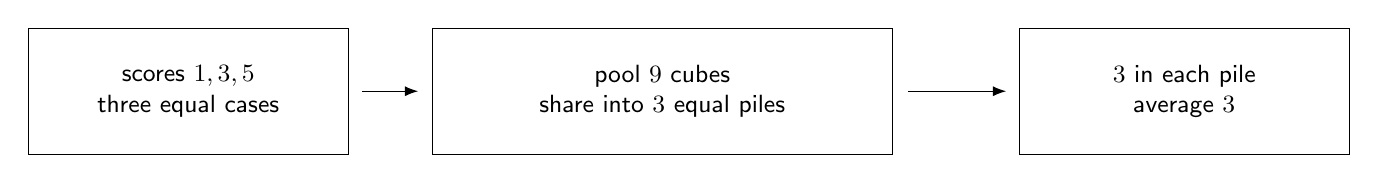
\begin{tikzpicture}[x=1in,y=1in,>=Latex,font=\small]
\node[draw,align=center,minimum width=1.6in,minimum height=0.63in] at (0.88,0.40)
 {scores $1,3,5$\\three equal cases};
\node[draw,align=center,minimum width=2.3in,minimum height=0.63in] at (3.25,0.40)
 {pool $9$ cubes\\share into $3$ equal piles};
\node[draw,align=center,minimum width=1.65in,minimum height=0.63in] at (5.86,0.40)
 {$3$ in each pile\\average $3$};
\draw[->] (1.75,0.40)--(2.03,0.40);
\draw[->] (4.48,0.40)--(4.97,0.40);
\end{tikzpicture}
\end{center}
The core remains available if this conversion needs more time. Fractions or
adult-supported equal-sized batch comparisons are needed here; notation is
optional, but averaging is part of the mathematics.

\task{5}{A current $4$ with two versus three offers left}
Both diagrams count the current offer; their two and three counters are not
numbers of \emph{future} offers. Taking $4$ gives average $4$ in either position.
\begin{center}
\begin{tabular}{@{}lccc@{}}\toprule
Offers left & Average if take & Best average if pass & Best choice \\\midrule
Two including this one & $4$ & $(0+4+6)/3=10/3$ & Take \\
Three including this one & $4$ & $40/9$ & Pass \\\bottomrule
\end{tabular}\end{center}
With two left, passing forces the next offer: its three-case total is $10$,
versus $12$ for three copies of a taken $4$. With three left, passing leaves
Problem 3's best two-offer rule and its nine-case total $40$, versus $36$ for
nine copies of $4$. The continuation includes another choice on the next offer.
Do not replace its value with the next single draw's mean.
\hint{(1) ``After you pass, how many counters will remain?''
(2) Set out the complete remaining one- or two-offer cards.
(3) Compare the continuation total with the same number of copies of score $4$.}

\task{6}{The best three-offer plan, including remembered histories}
\textbf{Answer:} first take only $6$; if continuing, on the second offer take
$4$ or $6$ and pass $0$; take the final offer. Total $134$ on the 27 words,
average $134/27$. The full score list is Plan B on guide page 5.

\textbf{Object-based bound for every legal plan.} Start at the end. The final
offer is compulsory. After \emph{any} passed history, the next tickets are still
$0,4,6$ with equal chances. For a second offer $0$, taking contributes $0$ to
its three possible final tails; passing contributes at most $10$. At second
$4$, taking gives $12$ versus passing $10$; at $6$, taking gives $18$ versus
$10$. Consequently the best remaining nine-word total is $10+12+18=40$
after \emph{each} first-offer history.

Now group the 27 words by the first offer. Taking first $0$, $4$ or $6$ gives
$0$, $36$ or $54$ respectively on its nine tails. Passing permits at most
$40$ in each group. The group bounds are therefore $40,40,54$, total $134$.
Plan B attains all three bounds. A memory-dependent rule may choose differently
after different first offers, but each group's future bag and bound are the
same. A rule cannot use its remembered past to see an unseen tail.
\hint{(1) ``What choices remain with one counter?''
(2) Solve the last two offers separately after each possible passed first offer.
(3) Compare the nine-word take and continuation totals in each first-offer group.}
It is fine to keep a checked candidate plan as a conjecture and return to the
bound on another visit. Recording ``B beats A'' is weaker than explaining
``no legal plan can exceed $134$''.

\newpage
\topic{Continuation / student page 7}
\task{8}{Three versus four offers from $0,5,6$}
This requires fractional continuation averages or supported comparison of
equivalent batches. Reuse the nine-card result from Problem 7, rather than
asking children to transcribe 81 words. Let them reconstruct the later choices
before revealing this answer table.
\begin{center}
\begin{tabular}{@{}cp{4.12in}c@{}}\toprule
Offers & Optimal plan & Average \\\midrule
Three & Take $5$ or $6$ at either nonfinal offer; pass $0$; final compulsory. & $143/27$ \\
Four & First take only $6$. After passing, use the three-offer plan above. & $448/81$ \\\bottomrule
\end{tabular}\end{center}
Here $V_1=11/3$, and Problem 7 gives $V_2=44/9$.
With three offers including a current $5$, taking wins because $5>44/9$.
The best three-offer average is
\[
 V_3=\frac{44/9+5+6}{3}=\frac{143}{27}.
\]
With four offers including a current $5$, passing wins because $143/27>5$.
At a first $0$, also pass; at a first $6$, take. Thus
\[
 V_4=\frac{143/27+143/27+6}{3}=\frac{448}{81}.
\]
On all 27 complete three-offer words, the three-offer plan scores one $0$,
thirteen $5$s and thirteen $6$s: total $143$. On all 81 four-offer words,
the four-offer plan scores two $0$s, 26 $5$s and 53 $6$s: total $448$.
The last three offers after either passed first $0$ or passed first $5$ each
contribute $143$ over their 27 tails; first $6$ contributes $27\cdot6=162$.
These are exact case totals, not a forecast for a short playing sample.

\hint{(1) ``What is your best remaining plan after passing the current $5$?''
(2) Use the new bag's two-offer total to value the remaining two offers.
(3) Compare $5$ with that continuation average; then repeat using three
remaining offers.}
Optional adult question: ``Does adding time make a middling offer easier or
harder to pass?'' Do not generalize one changed choice to every distribution.

\task{9}{Can one extra offer lower the optimum or leave it unchanged?}
\textbf{It cannot lower it.} In an $(n+1)$-offer round, pass the first offer
whatever it is, then use the old optimal $n$-offer plan. Independence and the
unchanged bag reproduce its old average. The new optimum is at least as good
as that legal plan. This argument works for any known finite bag of scores,
including duplicate tickets or negative scores.

\textbf{It can be unchanged:} if every ticket has the same score $c$, every legal
plan scores $c$, at every positive horizon. For example a bag $2,2,2$ has best
average $2$ with one, two or any number of offers.

\textbf{For a nonconstant finite bag, each extra offer strictly improves it.}
Let the smallest score be $a$ and largest $M$. The all-$a$ word has positive
probability and forces reward $a<M$ for every legal plan, while no reward can
exceed $M$. Hence $V_n<M$. The next offer has positive probability of being
$M$, so
\[
 V_{n+1}-V_n=\mathbb E[\max(X,V_n)-V_n]
             =\mathbb E[(X-V_n)_+]>0.
\]
In words: pass a new first offer if it is below the old average, but take it
if above. Taking the largest score sometimes gives a strict improvement.
The strict statement needs a finite horizon and a genuinely nonconstant bag.
\hint{(1) ``Could you ignore the new first offer?''
(2) Try a bag whose scores are all identical.
(3) For a varied bag, can every legal plan still be forced to get the smallest
score on some full word? Compare its average with the largest score.}

\newpage
\topic{Adult proof, sources and the next visit}
\textbf{Why the recurrence proves optimality.} At one remaining offer the reward
is forced, so the optimum before drawing is $\mathbb E[X]$. Suppose the best
average for $m-1$ offers is $V_{m-1}$ after every passed history. Independence
makes that future problem the same after observing any current $x$. Taking
gives $x$; passing allows at most $V_{m-1}$, attained by the earlier optimal
plan. Choose the larger, then average over $x$. This proves the recurrence
and an attainable bound for all legal histories by induction. A randomized
choice is a weighted average of taking and passing, so cannot exceed their
maximum. At equality any mixture is also optimal. On this week's distinct
three-ticket bags, only the two-offer $0,3,6$ middle choice is tied among the
student positions.

\textbf{Why complete words matter.} With $k$ equally likely tickets sampled
independently, each length-$n$ \emph{ticket} word has probability $k^{-n}$.
Stopping early leaves unseen tails in that collection. An accepted first offer
represents $k^{n-1}$ full words, not one case. Shortened stopped records have
different weights; do not average a list with one representative per stopped
record or per distinct score. With unequal probabilities, use product weights.
Duplicate-score tickets can share a numerical word but retain their multiplicity.

\textbf{Mathematical source.} Thomas S. Ferguson, \emph{Optimal Stopping and
Applications}, Chapter 2, printed p.~2.1 (PDF p.~1), equation (1): general
finite-horizon backward induction. Section 2.4, printed pp.~2.7--2.8 (PDF
pp.~7--8), distinguishes sampling without replacement from iid offers;
equation (6), p.~2.8, gives the common-distribution recursion used here.
Section 2.1, p.~2.2 (PDF p.~2), gives the different relative-rank, best-choice
secretary objective. Primary text:
\href{https://www.math.ucla.edu/~tom/Stopping/sr2.pdf}{math.ucla.edu/~tom/Stopping/sr2.pdf}.
The finite-ticket instances, student tasks and guide examples are original
applications of established mathematics.

\textbf{Teaching lessons actually found, and our inferences.}
\begin{itemize}
\item The organizer's \emph{Pattern Block Exercises -- Google Docs}, PDF p.~1,
starts with five minutes of handling, then pairs/trios. The first-year report
in the project README stresses concreteness and learning by doing.
Our brief handling period and legal demonstration adapt that precedent.
\item Givental, Nemirovskaya and Zakharevich, \emph{Math Circle by the Bay}
(AMS, 2018), Preface, printed pp.~viii--x (PDF pp.~9--11). These pages discuss
deep mathematical context, independent attempts, manipulatives, and changes
in pace and depth.
Our multiple-visit core/proof menu is an inference, not a session from the book.
\item Rozhkovskaya, \emph{Math Circles for Elementary School Students:
Berkeley 2009 and Manhattan 2011} (AMS, 2014), Lesson 7, ``At the lesson,''
items 1--2 (EPUB \texttt{OEBPS/part0017.xhtml}), reports likely missed legal
chords and engaged K'nex polygon building. Lesson 8, item 2
(\texttt{part0018.xhtml}), reports copying and coloring delays and instructor help.
Our partner-enforced deadline and supplied cards respond to those observations.
\end{itemize}
None of these sources prescribes this ticket activity, validates its physical
implementation, or establishes its age fit. The adaptation is unpiloted.
The current group record also reports a successful tiling session and a lamp
rule children struggled to retain; visible state and partner checks are our
response, not a tested remedy.

\textbf{Returning children.} Prior Weeks 24 and 42--46 include expected points,
replacement draws or complete histories, but not this same finite-score
acceptance task in the scoped research check. File presence is not evidence a
child used or mastered them. Ask what was actually used. A later visit can
finish the exact comparison, develop Problem 6's bound, or use Problems 8--9;
preserve the accepted mathematical destination while pacing flexibly.

\textbf{After the session, record} the date, children and pages actually used;
which handling rules required rescue; each fixed plan and one recoverable word
or drawing worth keeping; whether a claim was \emph{tried, conjectured, checked
on all cases, or explained}; and what children wanted to continue. Separate
observed behavior from hypotheses about its cause. Note actual prep/staffing
and any failed physical pretest. Save unfinished complete sets and labelled
totals for a return visit. Digital correctness is not physical rehearsal or
classroom evidence.

\end{document}
